\RequirePackage{pdfmanagement-testphase}
\DeclareDocumentMetadata{
    pdfversion=1.7,
}
\documentclass{../../fal_assignment}
\graphicspath{ {../../} }

\usepackage{enumitem}
\usepackage{pdflscape}
\setlist{nosep} % Make enumerate / itemize lists more closely spaced
\usepackage[T1]{fontenc} % http://tex.stackexchange.com/a/17858
\usepackage{url}
\usepackage{todonotes}

\title{Tinkering Audio}
\author{Dr Norah Lorway \& Dr Michael Scott}
\module{COMP120}

\begin{document}

\section*{COMP120 Tinkering Audio Contracts}

\paragraph{You have been contracted by the software development house \textit{ZigZag Demeanour} to prototype the acoustics for their next project. They are creating a series of small digital dioramas in preparation to develop an installation for a museum. They wish for these dioramas to have an element of interactive audio to them in an effort to impress the museums' stakeholders, a focus group of visitors to test the experiences, and their funders. They expect you to work in C\# Unity to implement these dioramas to complement their development pipeline.}

\paragraph{Below is an example of what the company intends to prototype:}

\begin{figure}[h]
\centering
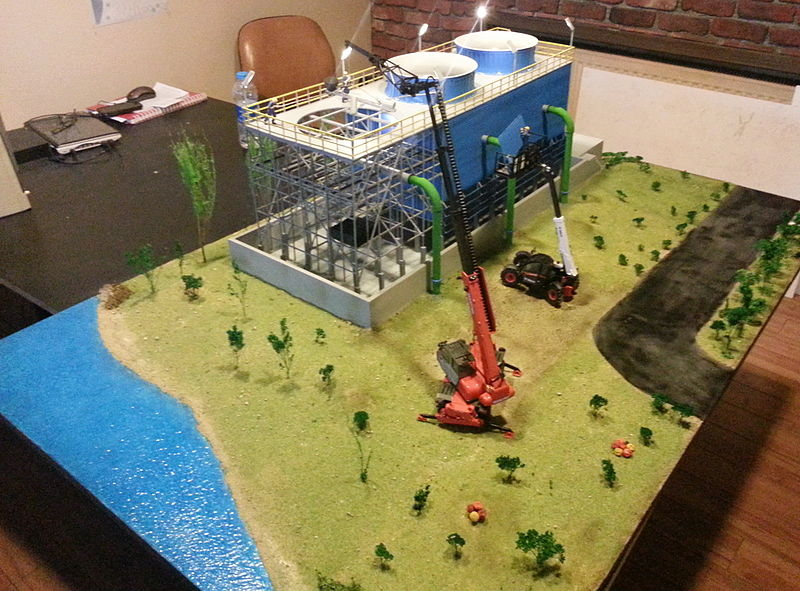
\includegraphics[width=6cm]{example_diorama}
\caption{An Example Diorama by Birhanb - \url{https://commons.wikimedia.org/wiki/File:Cooling\_tower\_construction\_diorama.jpg}}
\end{figure}

\paragraph{Please note the following constraints based on team composition:}

\paragraph{\textbf{Computing for Games} --- must be an interactive diorama that makes use of some element of physical simulation}

\paragraph{\textbf{Game Development} --- must be an interactive diorama that makes use of a character controller}

\paragraph{\textbf{Immersive Computing} --- must make use of an appropriate head-mounted display and teleportation to view the diorama}

\paragraph{\textbf{Robotics} --- must make use of an autonamous virtual robot with behaviours driven by a state-machine, sensing, and actuation that inhabits the diorama}

\paragraph{\textbf{Computer Science} --- must retrieve and process external online data source in real-time to affect the diorama in some way}

\paragraph{Additionally, the specific \textbf{ONE} diorama you and your group will devise and the associated form of tinkering audio will also depend on your team composition. Please see the Table on the next page.}

\begin{landscape}

\begin{table}[h]
\small
\begin{tabular}{l|l|llll|}
\cline{2-6}
                                                   & \textbf{Computing for Games}                                                         & \multicolumn{1}{l|}{\textbf{Game Development}}                                                             & \multicolumn{1}{l|}{\textbf{Immersive Computing}}                                                             & \multicolumn{1}{l|}{\textbf{Robotics}}                                                                      & \textbf{Computer Science}                                                           \\ \hline
\multicolumn{1}{|l|}{\textbf{Computing for Games}} & \begin{tabular}[c]{@{}l@{}}Manipulating Audio \\ (An Engine that Roars)\end{tabular} & \cellcolor[HTML]{9B9B9B}                                                                                   & \cellcolor[HTML]{9B9B9B}                                                                                      & \cellcolor[HTML]{9B9B9B}                                                                                    & \cellcolor[HTML]{9B9B9B}                                                            \\ \cline{1-3}
\multicolumn{1}{|l|}{\textbf{Game Development}}    & \begin{tabular}[c]{@{}l@{}}Weaving Audio\\ (A Spell that Collides)\end{tabular}      & \multicolumn{1}{l|}{\begin{tabular}[c]{@{}l@{}}Generating Audio \\ (An Ambience that Creeps)\end{tabular}} & \cellcolor[HTML]{9B9B9B}                                                                                      & \cellcolor[HTML]{9B9B9B}                                                                                    & \cellcolor[HTML]{9B9B9B}                                                            \\ \cline{1-4}
\multicolumn{1}{|l|}{\textbf{Immersive Computing}} & \begin{tabular}[c]{@{}l@{}}Rewriting Audio \\ (A Beat that Evolves)\end{tabular}     & \multicolumn{1}{l|}{\begin{tabular}[c]{@{}l@{}}Adapting Audio\\ (A Melody that Flows)\end{tabular}}        & \multicolumn{1}{l|}{\begin{tabular}[c]{@{}l@{}}Composing Audio \\ (An Instrument that Immerses)\end{tabular}} & \cellcolor[HTML]{9B9B9B}                                                                                    & \cellcolor[HTML]{9B9B9B}                                                            \\ \cline{1-5}
\multicolumn{1}{|l|}{\textbf{Robotics}}            & \begin{tabular}[c]{@{}l@{}}Affecting Audio\\ (A Reading that Inflexes)\end{tabular}  & \multicolumn{1}{l|}{\begin{tabular}[c]{@{}l@{}}Singing Audio\\ (A Bird that Ballads)\end{tabular}}         & \multicolumn{1}{l|}{\begin{tabular}[c]{@{}l@{}}Navigating Audio \\ (An Ear That Guides)\end{tabular}}         & \multicolumn{1}{l|}{\begin{tabular}[c]{@{}l@{}}Performing Audio \\ (A Robot that Expresses)\end{tabular}}   & \cellcolor[HTML]{9B9B9B}                                                            \\ \hline
\multicolumn{1}{|l|}{\textbf{Computer Science}}    & \begin{tabular}[c]{@{}l@{}}Converting Audio\\ (A Cityscape that Chants)\end{tabular} & \multicolumn{1}{l|}{\begin{tabular}[c]{@{}l@{}}Layering Audio\\ (A Hunt that Closes)\end{tabular}}         & \multicolumn{1}{l|}{\begin{tabular}[c]{@{}l@{}}Reverberating Audio\\ (A Chambre that Echos)\end{tabular}}     & \multicolumn{1}{l|}{\begin{tabular}[c]{@{}l@{}}Conducting Audio\\ (A Baton that Orchestrates)\end{tabular}} & \begin{tabular}[c]{@{}l@{}}Instructing Audio \\ (A Flute that Unlocks)\end{tabular} \\ \hline
\end{tabular}
\end{table}

\end{landscape}

\paragraph{It is up to you to determine what you make based on these prompts and the aforementioned constraints.}

\paragraph{Since the company is more interested in the technology, you have creative freedom to interpret the prompt in your own way.}

\paragraph{In considering the audio, there six general types of diorama to consider. They differ by their focus on diegetic (`in the world') or non-diegetic (`outside of the world') sound. They also differ by whether the audio in the diorama is driven by the viewer (i.e., the audience interacts with the diorama directly to produce/modify the audio), is responsive to the viewer (e.g., the audio changes based on the location of the viewer, events trigger by proximity, etc.), or it cycles (i.e., the diorama repeats the same cycle of audio regardless of what the audience is doing).}

\paragraph{As such, it is anticipated that any single individual diorama will be of only one type. It will either diagetic or non-diagetic sound---not both. It will either be viewer-driven, viewer-responsive, or cycling.}

\paragraph{Further to this, please carefully consider the algorithms you will use to generate and/or manipulate and/or combine audio. You needn't do all these things, but typically you will likely need multiple algorithms---whether these are generating and/or modifying and/or blending audio--- to implement a single feature.}

\paragraph{You are advised to manage scope carefully---this need only be a poof-of-concept. Simple is better.}

\end{document}